\documentclass{bredelebeamer}
\usepackage{multirow}
\usepackage{pdfpages}
\usepackage{braket,bigstrut}
\usepackage{palatino}
\usepackage{multicol,bigstrut}
\usepackage{listings}
% Tema escogido en este ejemplo

% Velos
\newtheorem{teo}{Teorema}
\newtheorem{ejemplo}{Ejemplo}
\newtheorem{defi}{Definici�n}
\newtheorem{coro}{Corolario}
\newtheorem{prueba}{Prueba}
\usepackage{tikz}
\usepackage{booktabs}
\usepackage{amsmath,amssymb,amsfonts,cancel}
\usetikzlibrary{positioning,shadows,backgrounds,calc}%
\def\Bb{{\bf{B}}}
\def\Db{{\bf{D}}}
\def\Eb{{\bf{E}}}
\def\Fb{{\bf{F}}}
\def\Kb{{\bf{k}}}
\def\Pb{{\bf{P}}}
\def\ab{{\bf a}}
\def\ib{{\bf{i}}}
\def\jb{{\bf{j}}}
\def\kb{{\bf{k}}}
\def\rb{{\bf r}}
\def\vb{{\bf v}}
\def\entonces{\;\;\;\Longrightarrow\;\;\;}
\newcommand{\der}[3][2]{\frac{d\! #2}{d\! #3}}
\newcommand{\ders}[3][2]{\frac{d^2\! #2}{d\! #3^2}}
\newcommand{\dert}[3][2]{\frac{d^3\! #2}{d\! #3^3}}
\newcommand{\derf}[3][2]{\frac{d^4\! #2}{d\! #3^4}}
\newcommand{\dern}[3][2]{\frac{d^n\! #2}{d\! #3^n}}
\newcommand{\dpr}[3][2]{\frac{\partial #2}{\partial #3}}
\newcommand{\dprs}[3][2]{\frac{\partial^2\! #2}{\partial #3^2}}
\newcommand{\dprt}[3][2]{\frac{\partial^3\! #2}{\partial\! #3^3}}
\newcommand{\dprf}[3][2]{\frac{\partial^4\! #2}{\partial\! #3^4}}
\newcommand{\dprn}[3][2]{\frac{\partial^n\! #2}{\partial\! #3^n}}
\newcommand{\dfr}[3][2]{\frac{\delta\! #2}{\delta\! #3}}
\newcommand{\dfrs}[3][2]{\frac{\delta^2\! #2}{\delta\! #3^2}}
\newcommand{\dfrt}[3][2]{\frac{\delta^3\! #2}{\delta\! #3^3}}
\newcommand{\dfrf}[3][2]{\frac{\delta^4\! #2}{\delta\! #3^4}}
\newcommand{\dfrn}[3][2]{\frac{\delta^n\! #2}{\delta\! #3^n}}
\newcommand{\abs}[1]{\left\vert#1\vphantom{y}\right\vert}%
\newcommand{\eva}[1]{\left.#1\vphantom{\frac yy}\right\vert}%
\newcommand{\cor}[1]{\left[ #1\vphantom{ y}\right]}
\newcommand{\fac}[1]{\left( #1\vphantom{y}\right)}


\setbeamercolor{footnote mark}{fg=black}
\setbeamercolor{footnote}{fg=black}


\renewcommand{\baselinestretch}{0.9}
\title[]{On the sensitivity reach of vector leptoquark production with preferential couplings to third generation fermions at the LHC}
\subtitle{}
\author[Cristian F. Rodr�guez]{
	A. Fl�rez\inst{1}, C. Rodriguez\inst{1}, J. Pe�uela-Parra\inst{1},\\
	J. Jones-P�rez\inst{2}, \\
	A. Gurrola\inst{3},
}

\institute[Uniandes]{\inst{1} Universidad de los Andes\and
\inst{2} Pontificia Universidad Cat�lica del Per� \and 
Vanderbilt University
}
\date{\today}
\lstset{language=C++,
  basicstyle=\ttfamily,
  keywordstyle=\color{blue}\ttfamily,
  stringstyle=\color{red}\ttfamily,
  commentstyle=\color{green}\ttfamily,
  morecomment=[l][\color{magenta}]{\#}
}
\usepackage[backend=bibtex8,style=authortitle,autocite=footnote]{biblatex}
\addbibresource{referencias.bib}

\renewbibmacro*{cite:title}{%
	\printtext[bibhyperref]{%
		\printfield[citetitle]{labeltitle}%
		\setunit{\space}%
		\printtext[parens]{\printdate}%
	}%
}

\renewcommand{\figurename}{{\bf Fig.}}
\usefonttheme{serif} % default family is serif
\newcommand{\PR}{{\pmb{P}_R}}

\newcommand{\PL}{{\pmb{P}_L}}
\definecolor{colordominante}{RGB}{11,17,79}
\definecolor{colordominanteF}{RGB}{219,68,14}
\definecolor{colorejemplo}{RGB}{77,190,208}
\definecolor{colordefinicion}{RGB}{0,51,102}
\definecolor{colorenfermedades}{RGB}{247,252,37}
\definecolor{colorteorema}{RGB}{0,133,202}
\definecolor{colortitulo}{RGB}{0,133,202}
\definecolor{colorcaja}{RGB}{230,050,030}
\definecolor{colorcajas}{RGB}{230,050,030}
\definecolor{grisamarillo}{RGB}{248,248,245} 
\definecolor{amarilloD}{RGB}{251,237,121}
\colorlet{colorfondoejemplo}{gray!10}
\colorlet{colorfondodefinicion}{gray!10}
\colorlet{colorfondoteorema}{gray!10}
\definecolor{colorfondocaja}{RGB}{252,252,244}

\definecolor{rosado}{RGB}{201,148,199}
\definecolor{violeta}{RGB}{117,107,177}
\definecolor{amarilloS}{RGB}{252,252,244}
\definecolor{azulF}{rgb}{.0,.0,.3}
\definecolor{grisD}{rgb}{.3,.3,.3}
\definecolor{grisF}{rgb}{.6,.6,.6}
\definecolor{miverde}{RGB}{44,162,67}
\usetikzlibrary{%
	matrix,
    decorations.pathreplacing,%
    decorations.pathmorphing,%
    decorations.markings,
    arrows,
    fadings,
%   arrows.meta,
    positioning,
    shapes,
    shadows,
    shapes.geometric
    }
		\usepackage{siunitx}
\definecolor{azulF}{rgb}{.0,.0,.3}
\definecolor{myblue1}{RGB}{0,157,209}
\definecolor{myblue2}{RGB}{161,224,255}
\definecolor{myblue3}{RGB}{216,229,245}
\definecolor{myblue4}{RGB}{0,149,229}

\tikzset{
  load/.style={
    ultra thick,
    -latex
  },  
  stress/.style={-latex},
 dim/.style={latex-latex},
  axis/.style={-latex,black!55},
  %
  startstop/.style={
    rectangle, 
    rounded corners=15pt, 
    minimum width=8cm, 
    minimum height=1cm,
    text centered, 
	font=\color{azulF}\sffamily, 
	fill=colorfondodefinicion!70!,
    line width=1pt,
    draw=colorejemplo!65!, 
  },  
 io/.style={
   trapezium, 
   trapezium left angle=70, 
   trapezium right angle=110, 
   minimum width=4cm, 
   minimum height=1cm, 
   text centered, 
	font=\color{azulF}\sffamily, 
	fill=colorfondodefinicion!70!,
    line width=1pt,
    draw=colorejemplo!65!, 
 },  
  process/.style={
    rectangle, 
     rounded corners, 
    minimum width=6cm, 
    minimum height=1cm, 
    text centered, 
    text width=6cm, 
	font=\color{azulF}\sffamily, 
	fill=colorfondodefinicion!70!,
    line width=1pt,
    draw=colorejemplo!65!, 
  },  
    process2/.style={
    rectangle, 
     rounded corners, 
    minimum width=5cm, 
    minimum height=1cm, 
    text centered, 
    text width=5cm, 
	font=\color{azulF}\sffamily, 
	fill=colorfondodefinicion!70!,
    line width=1pt,
    draw=colorejemplo!65!, 
  },     process3/.style={
    rectangle, 
     rounded corners, 
    minimum width=2cm, 
    minimum height=1cm, 
    text centered, 
    text width=2cm, 
	font=\color{azulF}\sffamily, 
	fill=colorfondodefinicion!70!,
    line width=1pt,
    draw=colorejemplo!65!, 
  },  
  decision/.style={
    diamond, 
    minimum width=2.5cm, 
    minimum height=1cm, 
    text width=2.5cm, 
    text centered, 
	font=\color{azulF}\sffamily, 
	fill=colorfondodefinicion!70!,
    line width=1pt,
    draw=colorejemplo!65!, 
  },  
     ragged border/.style={ decoration={random steps, segment length=1mm, amplitude=0.5mm},
           decorate,
   },
}
 \tikzstyle{arrow} = [thick,
    azulF,
    ->,
    >=stealth]
   \tikzfading[name=fade out,
  inner color=transparent!0, outer color=transparent!100]
  \tikzstyle arrowstyle=[scale=1]
\tikzstyle directed=[postaction={decorate,decoration={markings,
    mark=at position .65 with {\arrow[arrowstyle]{stealth}}}}]
\tikzstyle reverse directed=[postaction={decorate,decoration={markings,
    mark=at position .65 with {\arrowreversed[arrowstyle]{stealth};}}}]

\begin{document}

\frame{\titlepage}
\begin{frame}$ $
  \begin{small}
      \tableofcontents
  \end{small}
\end{frame}
%\frame{\tableofcontents}

\section{Motivation}
\subsection{Lepton Flavor Universality in the SM of Particle Physics}

\begin{frame}{Lepton Flavor Universality in the SM of Particle Physics}{What is it?}
	\begin{multicols*}{2}
		\begin{center}
			\includegraphics[width=.45\textwidth]{zoo_2.png}
		\end{center}
		\begin{center}
			\includegraphics[width=.49\textwidth]{Elementary_particle_interactions.png}
		\end{center}
	\textbf{Remark:} Weak bosons mix between quarks generation, Weak bosons mix the different generations of quarks via the CKM matrix, but this does not happen for leptons. This property of the model is known as lepton flavor universality (LFU)\footcite{Buonaura_2020}.
	\end{multicols*}

\end{frame}

\subsection[LFU-V]{Lepton Flavor Universality Violation}

\begin{frame}{New Physics in Lepton Flavor Universality Violation}{Hints on B-Anomalies}
	\begin{multicols*}{2}
		\begin{center}
			\includegraphics[width=.50\textwidth]{LFUV.png}
		\end{center} 
	$b \rightarrow s \mu^{+} \mu^{-}$ The fraction of branching ratios from B mesons to Kaons and a different pair lepton-antilepton shows a $5\sigma$ anomalie \footcite{Capdevila_2018,Aebischer2020}
	$$
	R_{K^{(*)}}=\frac{\operatorname{BR}\left(B \rightarrow K^{(*)} \mu^{+} \mu^{-}\right)}{\operatorname{BR}\left(B \rightarrow K^{(*)} e^{+} e^{-}\right)}
	$$
	$b \rightarrow c \ell \nu$ Similarly to $R\left(K^{(*)}\right)$, the ratios $R\left(D^{(*)}\right)$ show deviations from the SM predictions with a combined significance of about $3 \sigma$\footcite{Amhis_2021}, 
	$$
	R_{D^{(*)}}=\frac{\operatorname{BR}\left(B \rightarrow D^{(*)} \tau \nu\right)}{\operatorname{BR}\left(B \rightarrow D^{(*)} \ell^{e\mu} \nu\right)}
	$$
	\end{multicols*}

\end{frame}

\begin{frame}{New Physics in Lepton Flavor Universality Violation}{Another Hints}
	\begin{multicols*}{2}
		\begin{center}
			\includegraphics[width=.50\textwidth]{LFUV.png}
		\end{center} 
		The measurement of Fermilab's Muon g-2 experiment has presented an apparent discrepancy  with an accuracy of 4.2 $\sigma$ \footcite{arxiv.1311.2198, Abi_2021}.\vfill
		
		$q\bar q \mapsto e^+ e^-$ CMS experiment observed more very high-energetic electrons in proton-proton collisions compared to muons than expected \footcite{Sirunyan2021}.\vfill
		
		CCA. It has been observed that certain $\beta$decays happen less frequently than expected. This tension, called the Cabibbo Angle anomaly (CAA), displays a significance around $3 \sigma$ \footcite{PhysRevLett.125.111801,PhysRevC.102.045501}. 
		
	\end{multicols*}
	
\end{frame}

\subsection{Hints on third generation Fermions Physics}

\begin{frame}{Hints for New Physics}{Can we explain the anomalous vertex?}
	
	\begin{center}
		\includegraphics[width=.80\textwidth]{NP.png}
	\end{center}
	
\end{frame}

\begin{frame}{Hints for New Physics}{There are several purposes to solve B-Anomalies}
	In the standard model, the $b\mapsto s \ell\ell $ process is gived by 
	\begin{center}
		\includegraphics[width=.55\textwidth]{B_SM_3.png}
		\pause
		\includegraphics[width=.44\textwidth]{B_ZP_3.png}\\
		$$ $$
		$ $\\
		{\Large Is the $b\mapsto s \ell\ell $ anomaly caused by a Z' Boson?}
	\end{center}
\end{frame}

\begin{frame}{Hints for New Physics}{There are several purposes to solve B-Anomalies}
	In the standard model, the $b\mapsto s \ell\ell $ process is gived by 
\begin{center}
	\includegraphics[width=.55\textwidth]{B_SM_3.png}
	\includegraphics[width=.44\textwidth]{B_LQ_3.png}\\
	$$ $$
	$ $\\
	{\Large Is the anomaly caused by a leptoquark?}
\end{center}

\end{frame}

\begin{frame}{Hints for New Physics}{There are several purposes to solve B-Anomalies}
	And the others B-Meson Anomalies?
	\begin{center}
		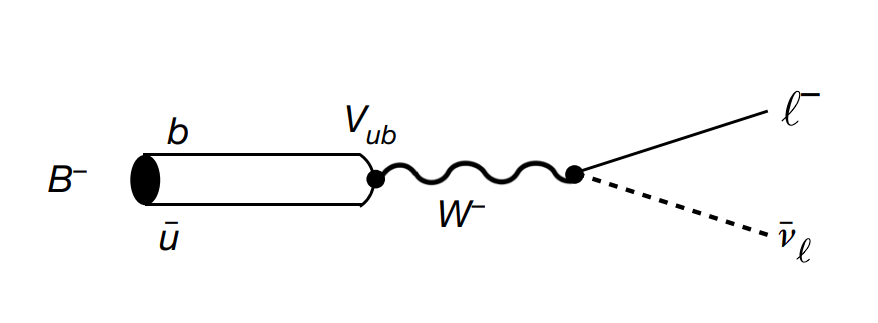
\includegraphics[width=.50\textwidth]{B_SM_1.png}
		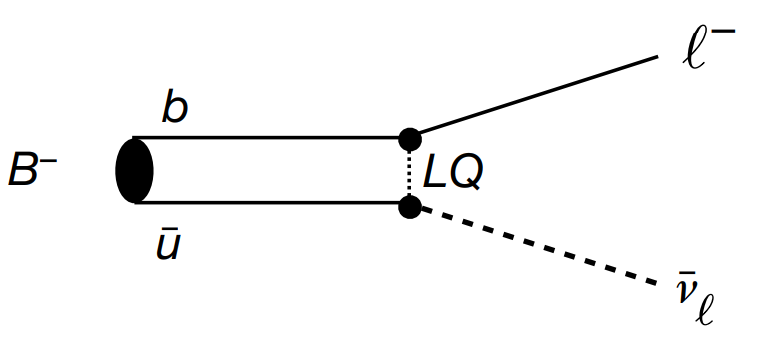
\includegraphics[width=.45\textwidth]{B_LQ_1.png}\\
		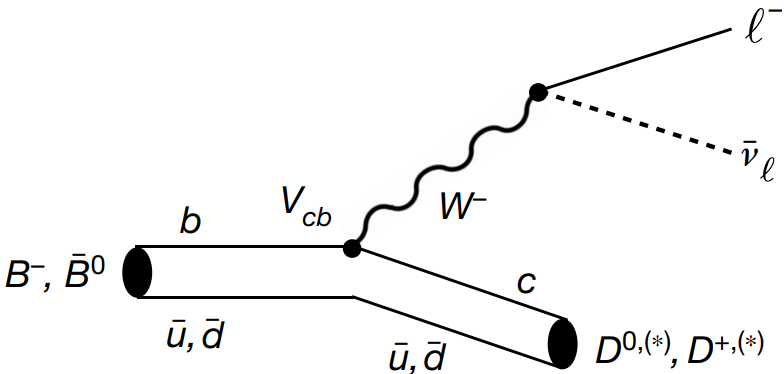
\includegraphics[width=.50\textwidth]{B_SM_2.png}
		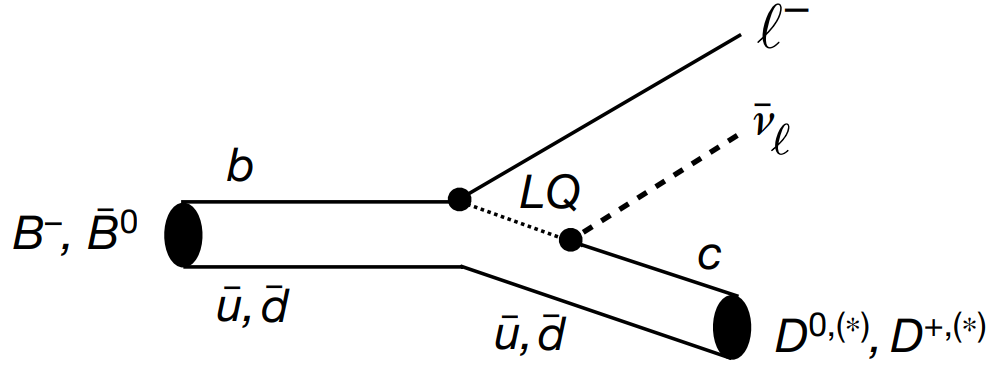
\includegraphics[width=.49\textwidth]{B_LQ_2.png}\\
		$$ $$
		$ $\\
		{\Large Is the $b\mapsto c \ell \nu  $ anomaly caused by a leptoquark?}
	\end{center}
\end{frame}


\begin{frame}{Hints for New Physics}{There are several purposes to solve B-Anomalies}

	\begin{center}
		\includegraphics[width=.85\textwidth]{B_WP.png}
		\\
		$ $\\
		{\Large Are the B-menson anomalies caused by a W' Boson?}
	\end{center}
\end{frame}

\begin{frame}{Hints for New Physics}{There are several purposes to solve B-Anomalies}
	\begin{center}
		\includegraphics[width=.85\textwidth]{B_3LQ.png}
		\\
		$ $\\
		{\Large Are the B-menson anomalies caused by three Leptoquarks?}
	\end{center}
	
\end{frame}

\begin{frame}{Hints for New Physics}{There are several purposes to solve B-Anomalies}
	\begin{center}
		\includegraphics[width=.89\textwidth]{B_Axions.png}
		\\
		$ $\\
		{\Large Are the B-menson and $g-2$ anomalies caused by axions?}
	\end{center}\pause
	$ $\hfill...and a long proposals' list behind.
\end{frame}

\begin{frame}{Research Problem}{What to do with these hints?}
\begin{multicols}{2}
	{\Large \textit{What production mechanisms have the potential to be observed at the LHC-experiments?}}\vfill
	\begin{enumerate}
		\item  Particles with preferred couplings to third generation fermions.\vfill
		\item  Compare exotic channels with dominant channels. 
		\vfill
		\item  We will use Machine Learning algorithms  to optimize data selection.
	\end{enumerate}
	
	\begin{center}
	\includegraphics[height=0.46\textheight]{pheno_2}
	\end{center}	
\end{multicols}
\end{frame}


\section[Searches for New Physics]{Searches for New Physics and Research Problem}
\begin{frame}{Large Hadron Collider}{How can we test these hypotheses?}
	\begin{multicols}{2}
		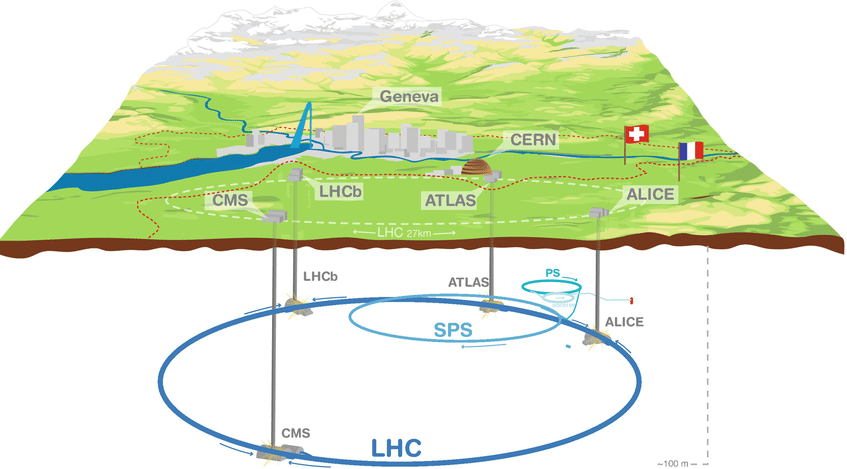
\includegraphics[width=.99\textwidth]{LHC.png}
	\end{multicols}
\begin{center}
	
\end{center}
\end{frame}


\begin{frame}{Multipurpose Detectors}{How can we test these hypotheses?}
	\begin{center}
		\includegraphics[width=.99\textwidth]{Detec.png}
	\end{center}
\end{frame}

\begin{frame}{Kinematic Variables}{How can we test these hypotheses?}
	\begin{center}
		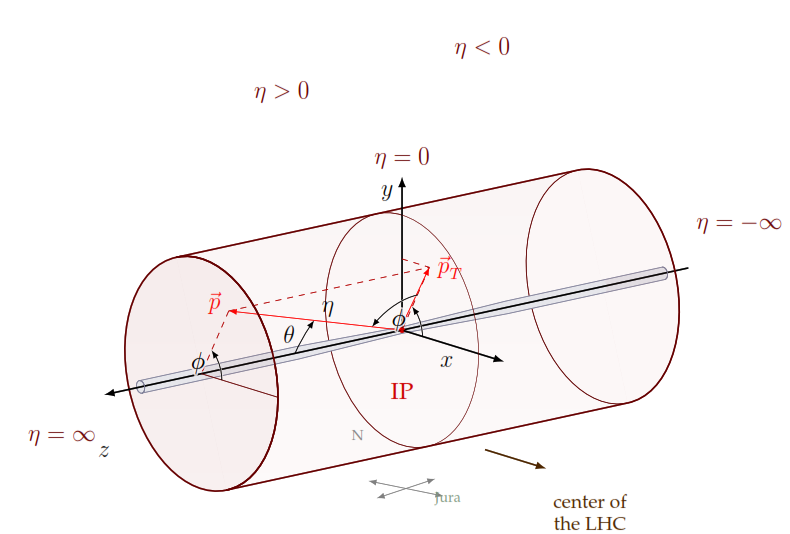
\includegraphics[width=.85\textwidth]{Kinematic_Variables.png}
	\end{center}
\end{frame}

\subsection{Searches for New Physics}
\begin{frame}{Hunting Peaks and Tails}{Searches for New Physics}
	\begin{multicols}{2}
		\includegraphics[width=.51\textwidth]{Higgs_CMS.png}\\
		$ $\\ \vfill
		One can construct a test that estimates how significant the deviation from the background in a distribution:
		$$
		s_{k}=\frac{N^{(obs)}-N^{(bkg)}}{\sigma_{N^{(bkg)}}}.
		$$
		It is said that a new discovery has $s_{k}\sim 5\sigma$.
		\vfill
		For MC events, if $S$ is the number of signal events expected and $B$ is the number of events coming from the background, we can then determine the significance of a Poissonic signal via the simple formula
		$$
		s_k=\frac{S}{\sqrt{S+B}}.
		$$
	\end{multicols}

\end{frame}

\section{Methodology}

\subsection[MC-Method]{Monte Carlo Method}
\begin{frame}{Montecarlo Generators}
	\begin{itemize}
		\item MonteCarlosimulation used to predict what we expect to see under certain conditions:
		\item To perform studies before having the data
		\item To compute event selection efficiency/acceptance
		\item  To predict the ammount and composition of background events
		\item To distinguish different signals. 
	\end{itemize}
	\begin{center}
		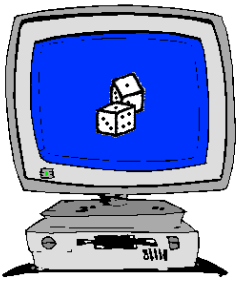
\includegraphics[scale=0.5]{A1}
	\end{center}
\end{frame}

\begin{frame}{Methodology}{What do we hope to simulate?}
	\begin{center}
		\includegraphics[width=.99\textwidth]{A2}
	\end{center}
\end{frame}
\subsection{Implementing Models}
\begin{frame}{The Toolchain}
	$\!\!\!\!\!\!\!\!\!\!\!\!\!\!\!\!\!\!\!\!\!\!\!\!\!\!\!\!\!\!\!\!\!\!\!\!$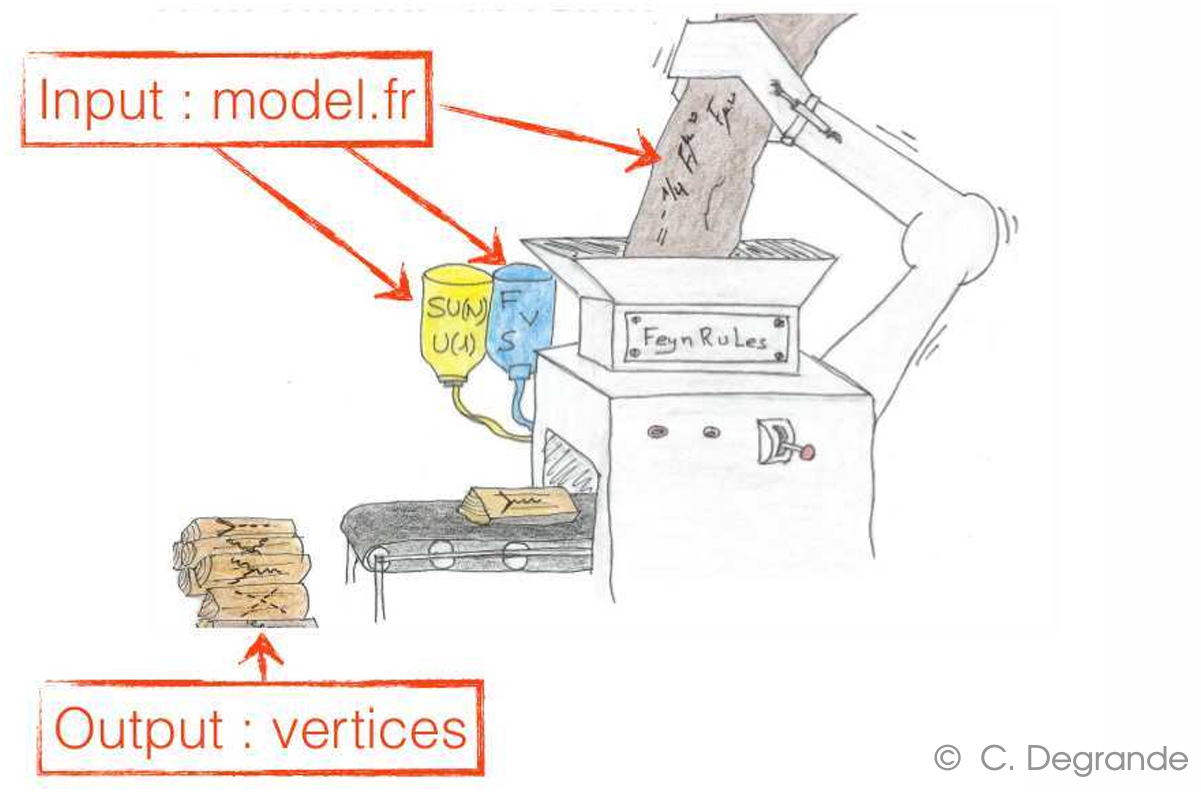
\includegraphics[width=1.33\textwidth]{Feynrules.pdf}

\end{frame}




\subsection[Objectives]{Research Objectives} 
\begin{frame}{Objectives and Methodology} 
	\begin{center}
		{\large Conduct feasibility studies for the LHC associated with the production of new hypothetical particles through different production mechanism and with preferential couplings to third generation fermions. }\pause
	\end{center}
\vspace{25pt}
	\textbf{Activities}
	\begin{itemize}
		\item Produce simulations of different background processes from the standard model using the LHC conditions. 
		\item  Study theoretical models considering the production of leptoquarks, $W'$ and $Z'$ with preferential couplings to third generation fermions. 
		\item Generate simulations for the production of the new hypothetical particles of interest to determine the production cross section, kinematics, topology under the LHC conditions. 
		\item Perform feasibility studies for the different signal models using Machine Learning methods.
	\end{itemize}
\end{frame}

\section[Leptoquarks]{Single Leptoquark Channel Feasibility}
\subsection{The Vector Leptoquark Lagrangian}
\begin{frame}{The Vector Leptoquark Lagrangian}{Single Leptoquark Channel Feasibility}
	\begin{multicols}{2}
	A leptoquark is defined as a particle with a vertex that mix vectors and quarks.
	\begin{center}
	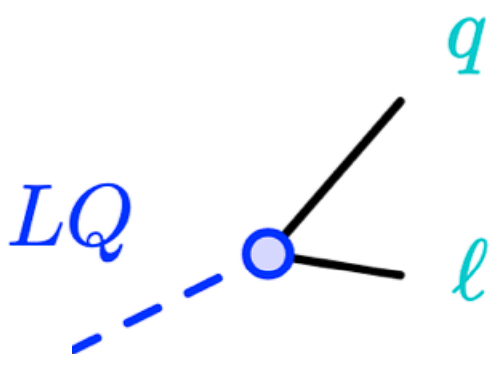
\includegraphics[width=.25\textwidth]{LQ_vertex.png}
	\end{center}
	If $U_1$ is a vector leptoquark that preserves the chirality on the vertex, we expect an interaction term like
	$$
	\sim U_1^\mu\bar{q}_{L} \gamma_{\mu} \ell_{L}
	$$
	
	Where the SM charges for the leptoquark must to be 
	\begin{tabular}{|c|c|c|c|c|}
		\hline & $\bar{q}_{L}$ & $\ell_{L}^{j}$ & $\bar{q}_{L}\gamma_{\mu} \ell_{L}$ & $U_{1}^{\mu}$ \\
		\hline$U(1)$ & $-1 / 3$ & $-1 $ & $-4 / 3$ & $+4 / 3$ \\
		\hline $\mathrm{SU}(2)$ & $\overline{\mathbf 2}$ & $\mathbf{2}$ & $\mathbf{1}$ & $\mathbf{1}$ \\
		\hline $\mathrm{SU}(3)$ & $\overline{\mathbf 3}$ & $\mathbf{1}$ & $\overline{\mathbf3}$ & $\mathbf{3}$ \\
		\hline
	\end{tabular}
\vfill
	And these allows a similar interaction term for the right handed currents 
	$$
	\sim U_1^\mu\bar{d}_{R} \gamma_{\mu} e_{R}.
	$$
	

	
	\end{multicols}

	
\end{frame}

\begin{frame}{The Vector Leptoquark Lagrangian}{Single Leptoquark Channel Feasibility}
	
	We consider a vector Leptoquark in a SM-representation  $\left(\mathbf{3}_{C}, \mathbf{1}_{I}, 2 / 3_{Y}\right)$
	\begin{align*}
		\mathcal{L}_{U}=&-\frac{1}{2} U_{\mu \nu}^{\dagger} U^{\mu \nu}+M_{U}^{2} U_{\mu}^{\dagger} U^{\mu}\\&-i g_{s}\left(1-\kappa_{c}\right) U_{\mu}^{\dagger} T^{a} U_{\nu} G^{\mu \nu}_a -\frac{2 i}{3} g'\left(1-\kappa_{Y}\right) U_{\mu}^{\dagger} U_{\nu} B^{\mu \nu}\\
		&+\frac{g_{U}}{\sqrt{2}}\left[U_{1}^{\mu}\left(\beta_{L}^{i j} \bar{q}_{L}^{i} \gamma_{\mu} e_{L}^{j}+\beta_{R}^{i j} \bar{d}_{R}^{i} \gamma_{\mu} e_{R}^{j}
		%+\beta_{N}^{i} \bar{u}_{R}^{i} \gamma_{\mu} N_{R}
		\right)+\text { h.c. }\right]
	\end{align*}
where $U_{\mu \nu}=\mathcal D_{\mu} U_{\nu}-\mathcal D_{\nu} U_{\mu}$, with $\mathcal D_{\mu}=\partial_{\mu}-i g_{s} G_{\mu}^{a} T^{a}-i \frac{2}{3} g_{Y} B_{\mu}$, and the couplings $\beta_{L}$ and $\beta_{R}$ are complex $3 \times 3$ matrices in flavor space:
	\begin{align*}
		&\beta_{L}=\left(\begin{array}{ccc}
			0 & 0 & \beta_{L}^{d \tau} \\
			0 & \beta_{L}^{s \mu} & \beta_{L}^{s \tau} \\
			0 & \beta_{L}^{b \mu} & 1
		\end{array}\right),  \beta_{R}=\left(\begin{array}{ccc}
			0 & 0 & 0 \\
			0 & 0 & 0 \\
			0 & 0 & \beta_{R}^{b \tau}
		\end{array}\right).
	\end{align*}
Where, we assume that the new vectors are coupled dominantly to third generation fermions.
\end{frame}

\subsection{Parameters to solve B-Anomalies}
\begin{frame}{Parameters to solve B-Anomalies}{Single Leptoquark Channel Feasibility}
	From \cite{Cornella2021}
\begin{center}$ $\hfill
	\includegraphics[width=.35\textwidth]{../RDwRHC}\hfill
\includegraphics[width=.35\textwidth]{../RDmixHC}\hfill$ $
\begin{tabular}{cccc}
	\hline
	\multicolumn{1}{c}{Scenario} & Parameter & best fit & 1 $\sigma$ \bigstrut\\
	\hline
	\multicolumn{1}{c}{\multirow{4}[2]{*}{max. RH currents\newline{}$\newline{}\left(\beta_{R}^{b \tau}=-1\right)\newline{}$}} & $C_U$ & 0.004  & [0.002,0.006] \bigstrut\\
	& $\beta_L^{b\mu}$ & -0.21 & [-0.25,-0.14] \bigstrut\\
	& $\beta_L^{s\tau}$ & 0.21  & [0.12,0.26] \bigstrut\\
	& $\beta_L^{s\mu}$ & 0.03 & [0.01,0.04] \bigstrut\\
	\hline
\end{tabular}%
\end{center}
where $C_{U} \equiv g_{U}^{2} v^{2} /\left(4 M_{U}^{2}\right)$.
\end{frame}

\subsection{Leptoquark Branching Ratios}
\begin{frame}{Leptoquark Branching Ratios}{Single Leptoquark Channel Feasibility}
Branching ratios of two body vector-leptoquark decay from the best fit for two scenarios $\beta_{R}^{b \tau}=0$ (left) and $\beta_{R}^{b \tau}=-1$ (right).	
\begin{center}
	\includegraphics[width=.49\textwidth]{../BRwRHC}
	\includegraphics[width=.49\textwidth]{../BRmixHC}
\end{center} 
We calculate the decay width for all the process $LQ\mapsto $all all in madgraph width the implementation in feynrules from \cite{Baker2019}.
\end{frame}


\subsection{Production Cross Section}
\begin{frame}{Production Cross Section}{Single Leptoquark Channel Feasibility}
	{Cross section for the production of leptoquarks in different channels in the context of the LHC with proton-proton collisions at $\sqrt s$=13TeV in both scenarios $\beta_{R}^{b \tau}=0$ (left) and $\beta_{R}^{b \tau}=-1$ (right).}
	\begin{center}
		\includegraphics[width=.45\textwidth]{../XSwRHC}
		\includegraphics[width=.45\textwidth]{../XSmixHC}
	\end{center}
	An additional Jet in single leptoquark has cross section similar to single leptoquark. Would we get a cleaner channel if the signal is associated with a jet?
\end{frame}

\begin{frame}{VBF-like production}{Single Leptoquark Channel Feasibility}
	Can we take advantage of the background suppression of a VBF-like channel?
	
	{Feynman diagram for a VBF-like production of a single leptoquark.}
\begin{multicols}{2}
	\begin{center}
	\includegraphics[width=.45\textwidth]{../d1.pdf}
	\end{center}
\begin{center}
	$ $\\
	$ $\\
	$ $
	\begin{tabular}{r|l}
	\hline \hline { Criteria } & { Constraint }\bigstrut \\
	$|\eta(b)|,|\eta(\tau)|$ & $<$ 2.5 \bigstrut\\
	$|\eta(j)|$ & $<$ 5.0 \bigstrut\\
	$|p_T(j)|,|p_T(b)|$ & $>$ 30 GeV\bigstrut \\		
	$|p_T(\tau)|$ & $>$ 20 GeV\bigstrut \\		
	\hline \hline
\end{tabular}
\end{center}

\end{multicols}
	\textbf{Remark}: Baker's implementation is not efficient, we have made modifications to take the dominant terms at the vertices:
	$$
	\sim U_1^\mu (\bar b_L \gamma_\mu \tau_L - \bar b_R \gamma_\mu \tau_R) + h.c.
	$$
	This in turn allows us to study separately the channels with a single leptoquark and pair production.
	

\end{frame}

\subsection{Partonic Kinematics}
\begin{frame}{Partonic Kinematics}
\begin{center}
Semi on-Shell Production ($B_W=15$):\\
\includegraphics[width=.39\textwidth]{../R_mass_parton}
\includegraphics[width=.39\textwidth]{../eta_j_parton}\\
Pure on-Shell Production ($B_W=1$):\\
\includegraphics[width=.39\textwidth]{../R_mass_parton_bw_1}
\includegraphics[width=.39\textwidth]{../eta_j_parton_bw_1}
\end{center}
\end{frame}
\subsection{Event Selection and signal composition}
\begin{frame}{Pre-Selection}{Single Leptoquark Channel Feasibility}
We propose a simple direct selection
\begin{itemize}
	\item  1 b-jet.
	\item  1 light-jet.
	\item  2 hadronic $\tau$.
\end{itemize}
\begin{multicols}{3}
	Conditions:
	\begin{enumerate}
		\item  At least 4 jets
		\item  At least 1 good jet
		\item  At least 2 good jets
		\item  At least 3 good jets
		\item  At least 4 good jets
		\item  At least 1 b-jet
		\item  At least 1 light-jet
		\item  At least 1 $\tau$-jet
		\item  At least 2 $\tau$-jet
	\end{enumerate}
	\includegraphics[width=.63\textwidth]{../cutflow}
\end{multicols}
\end{frame}

\begin{frame}{Efficiency and background composition}{Single Leptoquark Channel Feasibility}

The dominant backgrounds turn out to be t-tbar, W+jets and Z+jets.
\begin{center}
	\includegraphics[width=1.\linewidth]{bkg.png}
\end{center}
However, the MC statistic for V+jet events is not sufficient to properly train a discriminator algorithm. We will assume that the efficiency of the ttbar-trained discriminator is extendable to others.


\end{frame}

\subsection{Machine Learning Discrimination}
\begin{frame}{Event Discrimination}{Single Leptoquark Channel Feasibility}
The differentiation between signal and background is made via the kinematic and topological differences between signal and background. 
% TODO: \usepackage{graphicx} required
\begin{figure}
	\centering
	\includegraphics[width=0.48\linewidth]{../dPt_b_t1_hadron}
\includegraphics[width=0.48\linewidth]{../Pt_b_hadron}
\end{figure}
For example, pT for the b-jet is boosted due to the leptoquark mass, and this bjet is strongly correlated with the $\tau$'s.
	
\end{frame}
\begin{frame}{Machine Learning Discrimination}
	\begin{figure}
		\centering
		\includegraphics[width=0.8\linewidth]{discr}
	\end{figure}
	\begin{center}
	\begin{tabular}{l||rrrrrrrr} 
		\hline 
		Mass (GeV)& 500 & 1000 & 1500 & 2000 & 2500 & 3000 & 3500 \\
		\hline 
		\hline 
		$\epsilon_{signal} (\%)$& $89.98$ & $96.40$ & $97.80$ & $98.41$ & $98.30$ & $96.09$ & $83.05$ \\
		$\epsilon_{ttbar} (\%)$	& $7.73$ & $3.00$ & $1.54$ & $1.28$ & $1.71$ & $3.06$ & $9.60$
		\\\hline 
	\end{tabular}
\end{center}	
\end{frame}
\subsection{Significance Test}
\begin{frame}{Significance Test}{Single Leptoquark Channel Feasibility}
	Our selection with  hadronic taus shows an exclusion feasibility on a leptoquark mass of 1.4TeV at 150/fb, which is directly competitive with what is reported in CMS searches\footcite{2021136446}.
	\begin{center}
		\includegraphics[width=0.65\linewidth]{Significance}
    \end{center}
	Add semileptonic taus, fully leptonic, and channels without associated jets.
\end{frame}
\section[TimelLine]{Expected Results and TimeLine}
\begin{frame}{Expected Results and Timeline}{2022}
\begin{tabular}{|c|l|c|c|c|}
	\toprule
	\multirow{2}[4]{*}{Etapa} & \multicolumn{1}{c|}{Academic Period} & \multirow{2}[4]{*}{2022-10} & \multirow{2}[4]{*}{2022-19} & \multirow{2}[4]{*}{2022-20}   \\
	\cmidrule{2-2}          & \multicolumn{1}{c|}{Activity} &       &       &        \\
	\midrule
	\multirow{3}[6]{*}{Single Leptoquark} & Theoretical study of models & x     &       &     \\
	\cmidrule{2-5}          & MC for the production  & x     &       &     \\
	\cmidrule{2-5}          & Perform feasibility studies & x     & x     & x    \\
	\midrule
	\multirow{2}[6]{*}{W' } & Theoretical study of models &       &   x    & x   \\
	\cmidrule{2-5}          & MC for the production  &       &       & x     \\
	\bottomrule
\end{tabular}%0
\end{frame}

\begin{frame}{Expected Results and Timeline}{2023}
	\begin{tabular}{|c|l|c|c|c|}
		\toprule
		\multirow{2}[4]{*}{Etapa} & \multicolumn{1}{c|}{Academic Period} & \multirow{2}[4]{*}{2023-10} & \multirow{2}[4]{*}{2023-19} & \multirow{2}[4]{*}{2023-20}   \\
		\cmidrule{2-2}          & \multicolumn{1}{c|}{Activity} &       &       &        \\
		\midrule
		\multirow{3}[6]{*}{W'} & Theoretical study of models & x     &       &     \\
		\cmidrule{2-5}          & MC for the production  & x     &  x     &     \\
		\cmidrule{2-5}          & Perform feasibility studies &      & x     & x    \\
		\midrule
		Internship & Internship &       &       &     x \\
		\midrule
		Z', HN-VBF  & Theoretical study of models &       &       & x   \\
		\bottomrule
	\end{tabular}%0
\end{frame}

\begin{frame}{Expected Results and Timeline}{2024}
	\begin{tabular}{|c|l|c|c|c|}
		\toprule
		\multirow{2}[4]{*}{Etapa} & \multicolumn{1}{c|}{Academic Period} & \multirow{2}[4]{*}{2024-10} & \multirow{2}[4]{*}{2024-19} & \multirow{2}[4]{*}{2024-20}   \\
		\cmidrule{2-2}          & \multicolumn{1}{c|}{Activity} &       &       &        \\
		\midrule
		\multirow{3}[6]{*}{Z', HN-VBF} & Theoretical study of models & x     &       &     \\
		\cmidrule{2-5}          & MC for the production  & x     &  x     &     \\
		\cmidrule{2-5}          & Perform feasibility studies &      & x     & x    \\
		\midrule
		Thesis & Write &   x    &   x    &     x \\
		\bottomrule
	\end{tabular}%0
\end{frame}


\begin{frame}{Summary}
\begin{itemize}
	\item  The lepton flavour physics is a wide window to find physics beyond the standard model.\vfill
	\item  New particles with preferred couplings to third generation fermions can give clues in LFUV.\vfill
	\item  The Monte Carlo Method is one of the most useful tools in understanding experimental results and helps describe what the results of different models would look like.\vfill
	\item  Machine learning methods show that they have the potential to optimize and refine searches for new physics.
\end{itemize}
\end{frame}
\end{document}
\begin{frame}{Standard Model of Particle Physics}{How it Works?}
	
	\begin{multicols*}{2}
		Using the Lagrangian formulation for fields, it is an gauge-invariant theory of the group of internal symmetries
		$$SU(3)\times SU(2)\times U(1),$$
		Spontaneously broken from 
		$$SU(2)\times U(1)\mapsto U_{EM}(1),$$ 
		via the vev ($v$) of the Higgs Field $\phi$.
		
		\begin{center}
			\includegraphics[width=.51\textwidth]{lXueN.png}
		\end{center}
	\end{multicols*}
\end{frame}

\begin{frame}{Hunting Peaks and Tails}{How can we test these hypotheses?}
	\begin{center}
		\includegraphics[width=.55\textwidth]{Hunt_Peak.png}
		\includegraphics[width=.44\textwidth]{Hunt_Tail.png}
	\end{center}
	$ $\hfill{REHACER}
\end{frame}



\begin{frame}{Montecarlo Generators}{Software Stages}
	\begin{center}
		\includegraphics[width=.99\textwidth]{A3}
	\end{center}
\end{frame}
\begin{frame}{Montecarlo Generators}{Input/Outputs}
	\begin{center}
		\includegraphics[width=.99\textwidth]{A4}
	\end{center}
\end{frame}
\begin{frame}{Montecarlo Generators}{ROOT Analysis}
	\begin{center}
		\includegraphics[width=.99\textwidth]{A5}
	\end{center}
\end{frame}